\documentclass{article}
\usepackage[margin=0.95in]{geometry}
\usepackage{graphicx, hyperref, booktabs, array}

\title{Analyzing SEC 10-K Corporate Filings:\\ A FinBERT Approach}
\author{Alper Yıldırım}
\date{\today}

\begin{document}
\maketitle

\section{Introduction}

For economic growth and development, the efficient allocation of resources in financial markets is a crucial factor. The claim for the causal relationship from the development of financial markets to economic growth is widely discussed and dated back to 1910s. \cite{schumpeter1911} \cite{king1993finance} \cite{levine1997financial} Following this claim, the efficiency in the financial markets becomes an important question for economic sciences. In his seminal paper, Eugene Fama proposed the Efficient Markets Hypothesis (EMH), which posits that financial markets reflect all available information in prices immediately and fully. \cite{fama1970efficient} Nowadays, using NLP techniques such as sentiment analysis, extracting information from the financial documents with relevant asset prices, thus empirically testing the Efficient Markets Hypothesis such that estimating whether the new information is reflected in asset prices is a feasible task. As a preliminary part of this task, in this study, randomly sampled SEC 10-K filings from 2020 and 2021 will be classified to assess sentiment, using several NLP techniques.
\\ 

\section{Literature Review}

In his exhaustive literature survey, Ravula emphasized the studies conducted text analysis using ``Management's Discussion and Analysis'' parts of 10-K filings. \cite{ravula2021text} In this realm, Tao et al. developed several deep learning models such as RNNs and LSTMs to assess the informational value of MD\&A parts for the Initial Public Offerings. \cite{tao2018analysing} In a similar fashion, DeSola et al. also used MD\&A parts of corporate filings for financial text analysis, training variants of FinBERT models. \cite{desola2019finbert} \\

\noindent There are also studies that is compatible with the future prospects of this study, i.e., estimating the relationship between stock price movements and text classification of SEC 10-K filings. Ke et al. constructed their own procedure SESTM (``Sentiment Extraction via Screening and Topic Modeling'') that utilizes machine learning and econometric methods to reveal the association between financial news and stock price movements. \cite{ke2019predicting} Moreover, text analysis of financial disclosures is not confined to sentiment classification. For instance, Theil et al. utilized a lexicon-based approach using Loughran and McDonald Dictionary to assess linguistic uncertainty in 10-K filings and measured the association between linguistic uncertainty and stock price volatility. \cite{theil2018word} \\

\section{Data \& Methodology}

Publicly traded companies in the United States are obliged to present their 10-K filings to the Securities Exchange Commission (SEC) annually. While the 10-K filings could be lengthful texts, those filings contain information about their most recent profits, cash flow, operations and firm's future plans and projections. Since firms must follow strict guidelines formally in 10-K filings compared to annual reports, retrieving textual information from hundreds of firms is a more agible objective. The Item 7 of the 10-K filings is called ``Management's Discussion and Analysis'' in which the managers analyze firm's performance and invoke confidence in investors. Therefore, MD\&A parts of the 10-K filing are conformable text data for the purpose of this study. Furthermore, as the 10-K filings are lengthful and contain thousands of tokens, analyzing only MD\&A section is instrumental to overcome potential memory overflow (RAM) issues. Therefore, for the purpose of data collection, the \texttt{ExtractorAPI} of the \href{https://sec-api.io/}{SEC API} is used to retrieve MD\&A part of 400 corporate filings, which are randomly sampled from publicly traded companies in the U.S., published in 2020 and 2021. \\

\noindent In 2017, the cutting-edge Transformer architecture was introduced and since then, Transformer models are state-of-the-art in the field of NLP. One notable manifestation of this progress, BERT (Bidirectional Encoder Representations from Transformers), an encoding-only model offering a bidirectional context understanding capability, was unveiled by Google in 2018. \cite{devlin2018bert} Araci then developed FinBERT as a specialized variant of BERT for financial text analysis in 2019. \cite{araci2019finbert} In their study, Huang et al. offered another FinBERT model pre-trained on financial communication text with the total corpora size of 4.5 billion tokens, ``fine-tuned on 10,000 manually annotated sentences from analyst reports.'' \cite{huang2023finbert} In this study, Huang et al. (2022) and a fine-tuned version of FinBERT by the author were employed to analyze MD\&A parts of the sampled SEC 10-K filings, thereby harnessing the latest developments in financial sentiment analysis. Lastly, extracting last hidden states with FinBERT model, two feature extraction approaches were developed to test alternative approaches: with Random Forest Classifier and with a neural network.

\section{Results \& Discussion}

Both untuned and fine-tuned FinBERT models iterated over the SEC 10-K filings yielded fallacious results. It is worth noting that the relevant code snippets are syntactically working; however, it consistently produces the same output repetitively, due to an underlying semantic error potentially. Therefore, to establish a benchmark and compare the models, four different approaches were implemented using the \texttt{financial\_phrasebank} dataset: untuned FinBERT, fine-tuned FinBERT, feature extraction via FinBERT with a Random Forest Classifier and feature extraction via FinBERT with a vanilla Neural Network, respectively. I selected untuned FinBERT as a benchmark to be beat with alternatives approaches. I did not just do fine-tuning as task-specific training, but I have also used feature extraction since the number of data points are limited both in SEC 10-K filings and \texttt{financial\_phrasebank} as feature extraction requires less data for training compared to fine-tuning. Lastly, to assess the importance of capturing nonlinearities, I have conducted feature extraction with both Random Forest Classifier and a vanilla neural network.

\begin{table}[htbp]
    \centering
    \begin{tabular}{>{\bfseries}l c} % bold header and custom column specification
        \toprule
        Model & \textbf{Accuracy} \\
        \midrule[\heavyrulewidth]
        FinBERT - untuned & 0.87 \\
        FinBERT - fine-tuned & 0.92 \\
        Feature Extraction via Random Forest Classifier & 0.79 \\
        Feature Extraction via Vanilla Neural Network & 0.89 \\
        \bottomrule
    \end{tabular}
    \label{table:acc}
    \caption{Model Accuracies on \texttt{financial\_phrasebank}}
\end{table}

\noindent Table 1 shows that, among those models, while the fine-tuned FinBERT trained with financial news performed best in terms of model accuracy, the feature extraction via Random Forest Classifier performed worst. The confusion matrices are displayed in \hyperref[sec:appendix]{Appendix}. \\

\noindent A notable result discerning the poorly performed models is the mis-classification of a number of non-neutral texts as neutral by both untuned FinBERT and the Random Forest Classifier. This discrepancy may be caused from the fact of a subtle dataset imbalance, where the number of neutral texts were exceeding the positive or negative texts. Furthermore, Random Forest Classifier might underperformed compared to other models since Random Forest Classifier as a classification head does not capture nonlinearities in language as neural networks through their activation functions do. An alternative explanation might be that the Random Forest Classifier underperformed because of limited sequential information capability compared to Transformer models or a neutral network. \\

\noindent On the other hand, extracting features with FinBERT and using a vanilla neural network as classification head outperformed not only Random Forest Classifier, but also untuned FinBERT. One possible explanation is that the neural network was trained with the training data of \texttt{financial\_phrasebank}, that is, similar to a fine-tuning task, the neural network as classification head was trained for this specific task. Additionally, while the untuned FinBERT performed with fixed hyperparameters, I conducted an hyperparameter search loop over optimizers, learning rates, and batch sizes. \\

\noindent Last but not least, the remarkable accuracy attained by the fine-tuned FinBERT can be attributed to the fact that the model was fine-tuned on a training dataset of financial news, and then employed to predict test set of financial news. This highlights the effectiveness of fine-tuning for task-specific performance enhancements. However, it is indispensable to note again that the \texttt{financial\_phrasebank} dataset had a limited number of data points. Therefore, the satisfactory performance obtained through feature extraction with a vanilla neural network is a significant outcome. \\

\noindent In a follow-up study, after adjusting for the error in iterative classification, the association of sentiments expressed in SEC 10-K filings and asset prices can be empirically examined. Furthermore, considering that market sentiments are reflected in asset prices in cryptocurrency markets, an analogous analysis using Twitter data for cryptocurrency markets is a viable and promising task for further investigation.

\newpage

\bibliographystyle{apalike}
\bibliography{ref}

\newpage

\section*{Appendix}\label{sec:appendix}

\begin{figure}[!htbp]
    \centering
    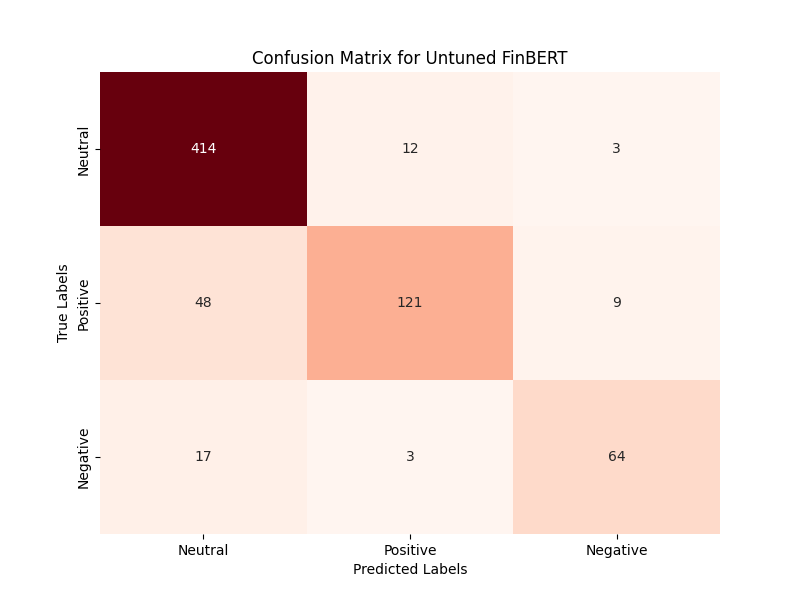
\includegraphics[width=0.75\textwidth]{assets/conf_mat_untuned.png}
    \caption{Confusion Matrix for ``yiyanghkust/finbert-tone''}
    \label{fig:untuned}
\end{figure}

\begin{figure}[!htbp]
    \centering
    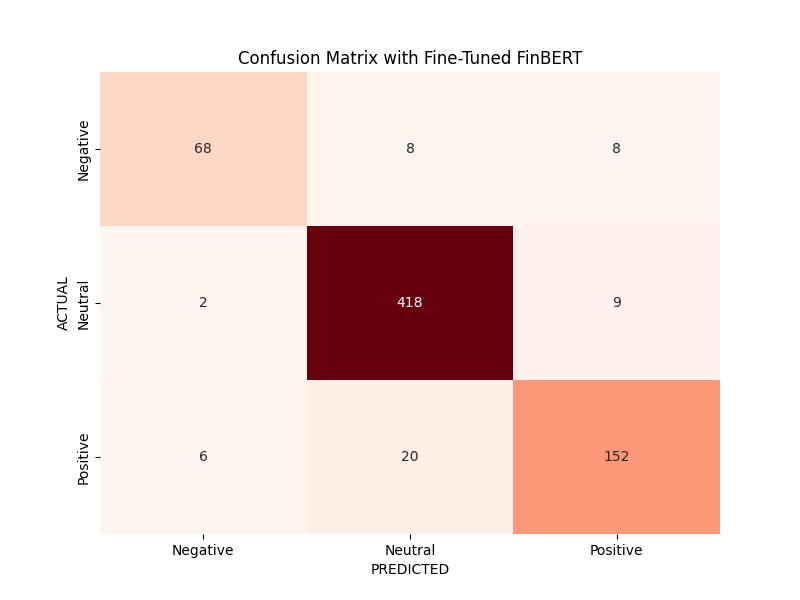
\includegraphics[width=0.75\textwidth]{assets/conf_mat_finetuned.png}
    \caption{Confusion Matrix for Fine-Tuned FinBERT}
    \label{fig:finetuned}
\end{figure}

\newpage 

\begin{figure}
    \centering
    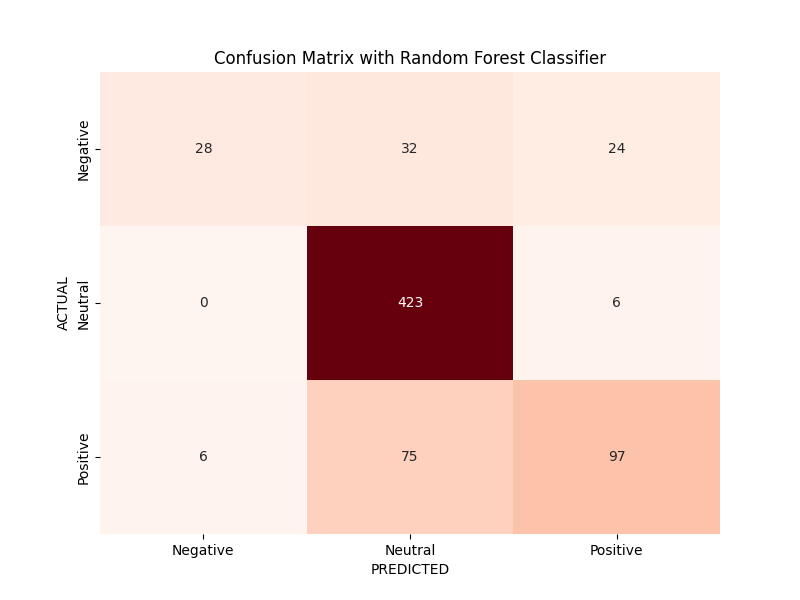
\includegraphics[width=0.75\textwidth]{assets/conf_mat_for_rfc.png}
    \caption{Confusion Matrix for Feature Extraction via Random Forest Classifier}
    \label{fig:rfc}
\end{figure}

\begin{figure}
    \centering
    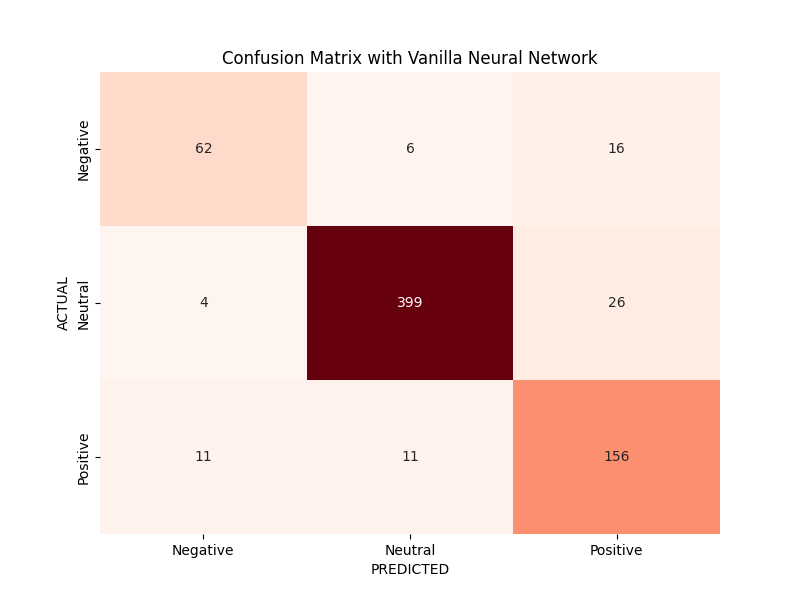
\includegraphics[width=0.75\textwidth]{assets/conf_mat_for_nn.png}
    \caption{Confusion Matrix for Feature Extraction via Vanilla Neural Network}
    \label{fig:nn}
\end{figure}

\end{document}